% RAG-Verify -- ICTCS 2026 submission (Springer LNNS proceedings).
% Built on the Springer Nature SVProc template supplied by the conference (svproc.cls v1.3, spmpsci.bst), both copied
% into this folder from latex-package.zip. Every number comes from results/ (see code/aggregate.py and
% code/check_paper.py --paper paper_ictcs); the table rows are copied from paper/tables by code/build_ictcs.py.
\documentclass{svproc}

% to typeset URLs, URIs, and DOIs (as in the template)
\usepackage{url}
\def\UrlFont{\rmfamily}
% Additions to the template: maths, table rules, scaling of the widest table, an algorithm float, sorted citations.
\usepackage{amsmath}
\usepackage{graphicx}
\usepackage{booktabs}
\usepackage{array}
\usepackage{algorithm}
\usepackage{algorithmic}
\usepackage{cite}
\usepackage{xcolor}

% \input inside a tabular breaks \multicolumn; the TeX primitive input does not.
\makeatletter\newcommand{\inputrows}{\@@input}\makeatother
\newcommand{\pending}{\textcolor{red}{\textsc{pend.}}}
\newcommand{\todo}[1]{\textcolor{red}{[PENDING: #1]}}
% ORCID iDs after author names, as in the Springer guidelines; Springer replaces them with the ORCID icon.
\newcommand{\orcidID}[1]{\textsuperscript{[#1]}}
% Scale a table down to the text width only when it is wider.
\newsavebox{\fitbox}
\newcommand{\fitwidth}[1]{\sbox{\fitbox}{#1}\ifdim\wd\fitbox>\textwidth\resizebox{\textwidth}{!}{\usebox{\fitbox}}\else\usebox{\fitbox}\fi}
% Let TeX stretch interword space a little rather than push long names and the URL into the margin.
\setlength{\emergencystretch}{2em}

\begin{document}
\mainmatter

\title{When Does Claim-Level Verification Help Small Retrieval-Augmented LLMs? An Empirical Study with RAG-Verify}
\titlerunning{Claim-Level Verification for Small Retrieval-Augmented LLMs}

% Names, affiliation and e-mails as in the authors' Information Fusion preprint; ORCID iDs supplied by the first
% author on 28 Oct 2026 (check digits verified). Author order and corresponding author set by the first author on
% 30 Oct 2026: Sengar, Sonawane, Joshi; corresponding author Bansidhar Joshi.
\author{Shivam Sengar\orcidID{0009-0007-4037-9595}
\and Yash Prabhakar Sonawane\orcidID{0009-0000-1556-4616}
\and Bansidhar Joshi\thanks{Corresponding author: \email{bansidhar11@gmail.com}}\orcidID{0000-0001-7141-7258}}
\authorrunning{S. Sengar et al.}
\tocauthor{Shivam Sengar, Yash Prabhakar Sonawane, and Bansidhar Joshi}

\institute{Department of Computer Science and Engineering,\\
Defence Institute of Advanced Technology (DIAT), Pune, Maharashtra, India\\
\email{shivamswngar4321@gmail.com}, \email{sonawaney789@gmail.com}, \email{bansidhar11@gmail.com}}

\maketitle

\begin{abstract}
Retrieval-augmented generation (RAG) reduces hallucination, yet small open models still give confident wrong answers when the retrieved evidence is incomplete. A popular remedy is a post-hoc check: split the answer into atomic claims, test each claim against the evidence, repair what fails, and abstain when the answer cannot be supported. This study asks whether this machinery earns its cost when the whole system must run on one 8\,GB consumer GPU. The proposed pipeline, RAG-Verify, combines a question-aware LLM check of the answer claim with natural language inference (NLI) on the remaining claims, followed by targeted revision and an abstention gate. It is compared with matched baselines on three disjoint 300-question test blocks of HotpotQA and TriviaQA using 4-bit Qwen2.5-7B and Llama-3.1-8B, with every design choice fixed beforehand on a separate development block. With Qwen2.5-7B, RAG-Verify cuts the hallucination rate of standard RAG from 50.6\% to 21.0\% on HotpotQA and from 23.8\% to 7.9\% on TriviaQA, and significantly raises effective reliability on both. However, a simpler baseline that asks the model to re-read the evidence and revise its answer once, with no verifier, is significantly better than RAG-Verify with Qwen and statistically tied with it with Llama, using fewer model calls. Trace analysis shows that the verifier flags 39\% of initially correct HotpotQA answers, and most flagged drafts end in abstention. At this scale, the benefit attributed to claim-level verification comes mainly from giving the model a second, evidence-focused pass.

\keywords{Large language models $\cdot$ Hallucination $\cdot$ Retrieval-augmented generation $\cdot$ Fact verification $\cdot$ Natural language inference $\cdot$ Selective question answering}
\end{abstract}

% =====================================================================
\section{Introduction}
Large language models (LLMs) produce fluent text that is not always true, a failure usually called hallucination~\cite{huang2023survey}. Retrieval-augmented generation (RAG), which grounds the model in retrieved passages~\cite{lewis2020rag,gao2023ragsurvey}, reduces the problem but does not remove it: the retriever can miss the decisive passage, and the model may ignore or misread evidence that is present~\cite{liu2023lost,niu2023ragtruth}. A growing family of methods therefore inspects the output after generation. Some plan and answer verification questions~\cite{dhuliawala2023cove}, some revise text using retrieved evidence~\cite{gao2022rarr}, some decompose an answer into atomic facts and test each one~\cite{min2023factscore,chern2023factool,wei2024safe,afev2025,vladika2025medical}, and others train the generator to critique its own retrievals~\cite{asai2023selfrag}.

Most of these studies use large proprietary models, yet many deployments must run locally, often on a single consumer graphics processing unit (GPU). There every extra model call costs latency, and claim decomposition, entailment checking and revision are themselves done by small models that make mistakes. It is not obvious that stacking these imperfect steps helps. This paper reports a controlled study of that question. We implement \emph{RAG-Verify}, a claim-level verify-and-revise pipeline built only from open models that fit in 8\,GB of GPU memory, and we compare it against baselines that share its retriever, prompts, and backbone but drop one ingredient at a time. Our contributions are:
\begin{enumerate}
\item A fully local claim-level verification pipeline with a \emph{hybrid} verifier: a question-aware LLM check for the claim that carries the answer and a natural language inference (NLI) model for the supporting claims.
\item A pre-registered protocol: the design is chosen on a held-out development block by a rule fixed in advance, and all systems are then run once on three disjoint test blocks per dataset, with paired bootstrap tests.
\item A negative but practically useful finding: an unconditional self-revision step with no verifier is significantly better than full claim-level verification on both datasets with Qwen2.5-7B and statistically tied with it with Llama-3.1-8B, with no more than 60\% of its model calls. A trace-level analysis locates the cause in verifier false alarms that convert correct answers into abstentions.
\end{enumerate}
Table~\ref{tab:abbr} lists the abbreviations used in the paper.

\begin{table}[htb]
\caption{Abbreviations used in this paper}
\label{tab:abbr}
\centering
\footnotesize
\setlength{\tabcolsep}{3pt}
\begin{tabular}{@{}l>{\raggedright\arraybackslash}p{4.55cm}l>{\raggedright\arraybackslash}p{4.55cm}@{}}
\toprule
Abbr. & Meaning & Abbr. & Meaning \\
\midrule
ANLI & Adversarial NLI dataset & LLM & Large language model \\
AUROC & Area under the receiver operating characteristic curve & MNLI & Multi-Genre NLI dataset \\
CI & Confidence interval & NF4 & 4-bit NormalFloat quantization \\
CoVe & Chain-of-Verification & NLI & Natural language inference \\
CRAG & Corrective RAG & Q4\_K\_M & 4-bit medium k-quant format of llama.cpp \\
F1 & Harmonic mean of precision and recall & RAG & Retrieval-augmented generation \\
FEVER & Fact Extraction and VERification dataset & RARR & Retrofit Attribution using Research and Revision \\
FLARE & Forward-Looking Active REtrieval augmented generation & SAFE & Search-Augmented Factuality Evaluator \\
GPU & Graphics processing unit & SQuAD & Stanford Question Answering Dataset \\
 & & WANLI & Worker-and-AI collaborative NLI dataset \\
\bottomrule
\end{tabular}
\end{table}

% =====================================================================
\section{Related Work}
\subsubsection{Retrieval and Adaptive Retrieval.} RAG conditions generation on passages from a dense or sparse retriever~\cite{lewis2020rag,gao2023ragsurvey}. FLARE~\cite{jiang2023flare} decides when to retrieve during generation, CRAG~\cite{yan2024crag} grades retrieved documents and falls back to other sources when they look unreliable, and Self-RAG~\cite{asai2023selfrag} trains the generator to emit reflection tokens that rate each passage's relevance and support and the usefulness of the output.

\subsubsection{Post-hoc Verification and Revision.} Chain-of-Verification (CoVe)~\cite{dhuliawala2023cove} drafts an answer, plans verification questions, answers them independently, and writes a final response. RARR~\cite{gao2022rarr} retrieves evidence for an existing output and edits unsupported spans. Claim-level pipelines such as FActScore~\cite{min2023factscore}, FacTool~\cite{chern2023factool}, and SAFE~\cite{wei2024safe} split text into atomic facts and check each one against a knowledge source; more recent work refines the decomposition step~\cite{afev2025}, applies atomic checking to medical RAG~\cite{vladika2025medical}, separates retrieval, verification and calibration into modules~\cite{r2vc2026}, or verifies entities against evidence~\cite{jia2026entity}. Lightweight checkers such as MiniCheck~\cite{tang2024minicheck} and NLI models trained on many entailment datasets~\cite{laurer2023nli,he2021debertav3} make claim checking affordable.

\subsubsection{Detection Without Retrieval, and Abstention.} SelfCheckGPT~\cite{manakul2023selfcheckgpt} and semantic entropy~\cite{farquhar2024semantic} detect hallucinations from disagreement between samples. Benchmarks such as HaluEval~\cite{li2023halueval}, TruthfulQA~\cite{lin2021truthfulqa}, RAGTruth~\cite{niu2023ragtruth} and FaithJudge~\cite{tamber2025faithjudge} measure the problem. Declining to answer is a legitimate outcome when the model is unsure~\cite{wen2024abstention}; we therefore score systems by effective reliability~\cite{whitehead2022reliable}, defined in Sect.~\ref{sec:setup}. Our study differs from this work in scope rather than mechanism: one consumer GPU, the simple baselines a deployer would try first, and the contribution of each component.

% =====================================================================
\section{Method}
\subsection{Pipeline}
Given a question $q$, a retriever $R$ returns the top-$k$ passages $P=\{p_1,\dots,p_k\}$, and the generator LLM $G$ produces a short response $r_0$ in a fixed format (answer line plus one-sentence explanation). RAG-Verify splits $r_0$ into $m$ atomic claims $C=(c_1,\dots,c_m)$, where the \emph{answer claim} $c_1$ states the answer, and gives each claim $c_i$ a label $\ell_i\in\{\textsc{supported},\textsc{contradicted},\textsc{unsupported}\}$; $\ell=(\ell_1,\dots,\ell_m)$ denotes the list of labels. If some claim is not supported, $G$ writes a revised response $r_1$. Two parameters steer the decisions: the entailment threshold $\tau$ of the NLI model $N$, and the minimum fraction $\rho$ of supported claims that an answer needs. Algorithm~\ref{alg:rv} gives the steps.

\begin{algorithm}[htb]
\caption{RAG-Verify (one question)}\label{alg:rv}
\begin{algorithmic}[1]
\REQUIRE $q$, $R$, $G$, $N$, $\tau$, $\rho$
\STATE $P \gets R(q,k)$; \quad $r_0 \gets G(\textsc{Answer}(q,P))$
\STATE $C \gets \textsc{Decompose}_G(q,r_0)$ \COMMENT{answer claim first}
\STATE $\ell \gets \textsc{Verify}(q,C,P)$ \COMMENT{hybrid, Eq.~(\ref{eq:label})}
\STATE $r_1 \gets r_0$
\IF{some $\ell_i \neq \textsc{supported}$}
  \STATE $r_1 \gets G(\textsc{Revise}(q,P,r_0,\{(c_i,\ell_i)\}))$
  \IF{$r_1$ is a refusal (``I don't know'')}
    \RETURN \textsc{abstain}
  \ENDIF
  \STATE $C \gets \textsc{Decompose}_G(q,r_1)$; \quad $\ell \gets \textsc{Verify}(q,C,P)$
\ENDIF
\IF{$\ell_1 \neq \textsc{supported}$ \textbf{or} $s(\ell) < \rho$}
  \RETURN \textsc{abstain}
\ENDIF
\RETURN the answer in $r_1$
\end{algorithmic}
\end{algorithm}

\subsubsection{Decomposition.} $G$ is prompted with two worked examples to rewrite the response as at most twelve self-contained atomic claims ($m\le 12$), the first of which must state the answer. Because small models do not always respect that ordering, we move the claim that contains the answer string $a$ (the answer line of the response) to the front, or insert the template claim \emph{``The answer to the question `$q$' is $a$''} when no claim contains it.

\subsubsection{Hybrid Verification.} For a supporting claim $c_i$ ($i>1$), $N$ returns entailment and contradiction probabilities for each premise; premises are the $k$ passages plus the concatenation of the top three, which allows two-hop facts to be entailed. With $e_i$ and $x_i$ the highest entailment and contradiction probabilities over all premises, the label is
\begin{equation}
\ell_i=\begin{cases}\textsc{supported} & e_i\ge\tau\\ \textsc{contradicted} & e_i<\tau,\ x_i\ge\tau\\ \textsc{unsupported} & \text{otherwise.}\end{cases}\label{eq:label}
\end{equation}
For the answer claim $c_1$ we do not use NLI. On the development block we observed that NLI entailed claims such as ``the answer is $X$'' whenever $X$ appeared in a passage, even when $X$ answered a different question; it caught only 3 of 17 wrong answers in a manual check, against 7 of 17 for an LLM judge. The answer claim is therefore judged by $G$ itself with a prompt that asks whether the proposed answer is correct \emph{for this question} given the passages.

\subsubsection{Revision and Abstention.} Flagged claims and their labels are shown to $G$ together with the passages and the original response; $G$ may correct the answer or reply that it does not know. After re-verification, the system abstains if the answer claim is not supported or if the supported fraction
\begin{equation}
s(\ell)=\frac{1}{m}\sum_{i=1}^{m}\mathbf{1}[\ell_i=\textsc{supported}]
\end{equation}
falls below $\rho$, where $\mathbf{1}[\cdot]$ is 1 when its condition holds and 0 otherwise.

\subsection{Design Selection on Development Data}
Before any test run we fixed the selection rule: maximize mean effective reliability over the two development blocks (100 questions each), breaking ties within 0.01 by higher coverage, then fewer model calls, then $\tau$ closest to 0.5. We compared three verifiers (NLI only, hybrid, LLM judge for every claim), $\tau\in\{0.3,0.5,0.7,0.9\}$, and $\rho\in[0,1]$ (simulated offline from saved scores). The rule selected the hybrid verifier with $\tau=0.3$ and $\rho=0$, i.e., abstention is driven by the answer claim alone; mean development reliability was 0.200. This frozen configuration is reported as RAG-Verify.

% =====================================================================
\section{Experimental Setup}\label{sec:setup}
\subsubsection{Data.} We use HotpotQA (distractor setting, validation split)~\cite{yang2018hotpotqa} and the Wikipedia subset of TriviaQA (validation split)~\cite{joshi2017triviaqa}. A fixed permutation (seed 2026) of each split gives three disjoint 300-question test blocks and one 100-question development block. Retrieval corpora are built from the provided contexts: 66{,}635 unique HotpotQA paragraphs from all 7{,}405 validation questions, and 135{,}517 100-word passages from 3{,}120 TriviaQA evidence pages (the 1{,}000 sampled questions plus 1{,}100 distractor questions). These are closed corpora, not full Wikipedia, so absolute scores are not comparable to open-domain results. To test the verifiers in isolation we also use HaluEval-QA~\cite{li2023halueval}: 1{,}000 questions sampled with the same seed, each with its gold knowledge snippet and one correct and one hallucinated answer (2{,}000 items).

\subsubsection{Models.} We use two instruction-tuned generators, Qwen2.5-7B-Instruct~\cite{qwen2024qwen25} and Llama-3.1-8B-Instruct~\cite{dubey2024llama3}, both 4-bit (Q4\_K\_M) served by Ollama with temperature 0, a fixed seed, and an 8{,}192-token context. The retriever is bge-small-en-v1.5~\cite{xiao2023cpack} with exact inner-product search, $k=5$. The NLI model is the DeBERTa-v3-large~\cite{he2021debertav3} checkpoint of Laurer et al.~\cite{laurer2023nli}, fine-tuned on MNLI, FEVER~\cite{thorne2018fever}, ANLI, LingNLI and WANLI. Self-RAG uses the authors' 7B checkpoint~\cite{asai2023selfrag} quantized to 4-bit NF4. Hardware is a laptop with an RTX~4060 (8\,GB).

\subsubsection{Systems.} All retrieval-based systems share the same retriever, passages, and answer format. \emph{Closed-book} answers without passages. \emph{Standard RAG} answers from the passages. \emph{RAG + abstain prompt} adds an instruction to reply ``I don't know'' when the passages are insufficient. \emph{RAG + self-revision} (RAG-Verify without the verifier) shows the model its first response and the passages and asks it to correct any error or abstain. \emph{CoVe}~\cite{dhuliawala2023cove} uses the factored variant with up to five verification questions, either closed-book or with retrieval for every verification question. \emph{Self-RAG}~\cite{asai2023selfrag} follows the authors' short-form inference (adaptive retrieval threshold 0.2, equal weights for the critique scores).

\subsubsection{Metrics.} An answer is correct if, after SQuAD normalization~\cite{rajpurkar2016squad}, it equals or contains a gold alias. For a set of $n$ questions, let $A$ be the accuracy (fraction answered correctly) and $H$ the hallucination rate (fraction answered incorrectly); abstentions count towards neither. Effective reliability~\cite{whitehead2022reliable} with unit cost rewards a correct answer, penalizes a wrong one, and gives zero to an abstention:
\begin{equation}
\Phi_1 = A - H = \frac{1}{n}\sum_{j=1}^{n}\begin{cases}+1 & \text{question $j$ answered correctly}\\ -1 & \text{question $j$ answered wrongly}\\ 0 & \text{question $j$ abstained.}\end{cases}
\end{equation}
We report mean $\pm$ standard deviation over the three test blocks, and paired bootstrap 95\% confidence intervals (CIs; 10{,}000 resamples) over the 900 pooled questions. On the first test block we also measure FActScore-style claim precision of answered outputs: a fixed extractor (Llama-3.1-8B for every system) splits each output into atomic claims, and MiniCheck-Flan-T5-Large~\cite{tang2024minicheck} judges each claim against gold evidence (HotpotQA supporting paragraphs; for TriviaQA, the five gold-page chunks closest to the claim). Latency is the median wall-clock time per question on the first 50 development questions, with one system on the GPU at a time.

% =====================================================================
\section{Results}
\begin{table}[htb]
\caption{Test results (\%, mean $\pm$ standard deviation over three disjoint 300-question blocks). Acc: accuracy; Abst: abstention rate; Hall: answered and wrong; $\Phi_1$: effective reliability (higher is better)}
\label{tab:main}
\centering
\setlength{\tabcolsep}{3pt}
\fitwidth{%
\begin{tabular}{lcccccccc}
\toprule
 & \multicolumn{4}{c}{HotpotQA} & \multicolumn{4}{c}{TriviaQA} \\
\cmidrule(lr){2-5}\cmidrule(lr){6-9}
System & Acc$\uparrow$ & Abst & Hall$\downarrow$ & $\Phi_1\uparrow$ & Acc$\uparrow$ & Abst & Hall$\downarrow$ & $\Phi_1\uparrow$ \\
\midrule
\inputrows tables/main_rows.tex
\bottomrule
\end{tabular}}
\end{table}

\begin{table}[htb]
\caption{Paired bootstrap differences in $\Phi_1$ (percentage points, 95\% CI, 900 questions per dataset). (Q): Qwen2.5-7B backbone; (L): Llama-3.1-8B backbone; $^{*}$: CI excludes zero}
\label{tab:tests}
\centering
\setlength{\tabcolsep}{4pt}
\fitwidth{%
\begin{tabular}{lcc}
\toprule
Comparison & HotpotQA & TriviaQA \\
\midrule
\inputrows tables/tests_rows.tex
\bottomrule
\end{tabular}}
\end{table}

\subsubsection{Retrieval Matters Most.} Table~\ref{tab:main} lists all systems and Table~\ref{tab:tests} the paired comparisons. With Qwen2.5-7B, retrieval raises accuracy from 21.9\% to 47.4\% on HotpotQA and from 57.2\% to 75.6\% on TriviaQA. Closed-book CoVe does not improve on the closed-book model (21.8\% and 60.7\%), and CoVe with retrieval is close to standard RAG ($\Phi_1$ $-$2.0 vs.\ $-$3.1 on HotpotQA, 54.8 vs.\ 51.8 on TriviaQA) while making about 7.7 model calls per question: the same small model rarely overturns its own first answer.

\subsubsection{RAG-Verify Trades Coverage for Precision.} RAG-Verify lowers the hallucination rate of standard RAG from 50.6\% to 21.0\% on HotpotQA and from 23.8\% to 7.9\% on TriviaQA, the lowest of all systems on both datasets. It abstains on 49.2\% and 27.4\% of questions, so accuracy falls to 29.8\% and 64.7\%. The net effect on $\Phi_1$ is positive and significant: $+$11.9 points on HotpotQA and $+$5.0 on TriviaQA. When it does answer, RAG-Verify is right 58.5\% (HotpotQA) and 89.1\% (TriviaQA) of the time, against 48.4\% and 76.1\% for standard RAG.

\begin{figure}[htb]
\centering
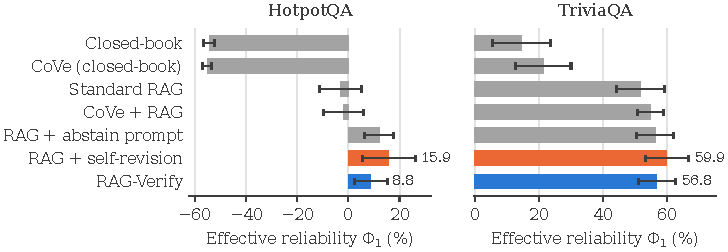
\includegraphics[width=\textwidth]{figures/phi1.pdf}
\caption{Effective reliability $\Phi_1$ of the Qwen2.5-7B systems (mean $\pm$ standard deviation over the three test blocks); self-revision and RAG-Verify are highlighted}
\label{fig:phi1}
\end{figure}

\subsubsection{Simple Baselines Are as Good or Better.} Fig.~\ref{fig:phi1} compares $\Phi_1$ across systems. A one-line abstention instruction already reaches $\Phi_1$ of 12.0 and 56.2; the difference from RAG-Verify is not significant on either dataset. Unconditional self-revision does better still: 15.9 on HotpotQA and 59.9 on TriviaQA, significantly above both RAG-Verify ($-$7.1 and $-$3.1 points for RAG-Verify) and the abstention prompt ($+$3.9 and $+$3.7). Self-revision makes exactly two model calls per question, whereas RAG-Verify makes 3.7 (HotpotQA) and 3.4 (TriviaQA) calls on average plus NLI inference.

\subsubsection{Backbone.} With Llama-3.1-8B the closed-book model is much stronger on TriviaQA (74.9\% vs.\ 57.2\%), so retrieval adds less (77.4\%), and the abstention prompt is followed less often (13.9\% and 9.9\% abstention vs.\ 34.0\% and 22.9\% for Qwen). RAG-Verify again beats standard RAG significantly ($\Phi_1$ $+$7.4 and $+$4.3 points) and again has the lowest hallucination rate among Llama systems (31.4\% and 11.6\%). Unlike with Qwen, self-revision is not better: the two are statistically tied on both datasets (8.1 vs.\ 6.4 on HotpotQA, 61.8 vs.\ 61.4 on TriviaQA), as are RAG-Verify and the abstention prompt, but RAG-Verify needs 5.2 and 4.9 model calls per question against two. Self-RAG answers almost every question (0.8\% and 0.6\% abstention) and has the highest hallucination rate of the retrieval-based systems (59.4\% and 25.7\%; $\Phi_1$ $-$19.7 and 48.1); this comparison is only indicative, as its backbone and quantization differ from ours.

% =====================================================================
\section{Analysis}
\begin{table}[htb]
\caption{Breakdown of RAG-Verify's decisions, computed from the saved traces (Qwen2.5-7B, 900 test questions per dataset)}
\label{tab:trace}
\centering
\begin{tabular}{lrr}
\toprule
 & HotpotQA & TriviaQA \\
\midrule
First draft correct & 425 & 682 \\
First draft flagged by verifier & 466 & 282 \\
\quad of which first draft was correct & 164 & 134 \\
Abstained: model refused in first draft & 19 & 7 \\
Abstained: model refused after revision & 380 & 233 \\
Abstained: final gate (answer claim) & 44 & 7 \\
\quad of which withheld answer was correct & 24 & 3 \\
Answered & 457 & 653 \\
\bottomrule
\end{tabular}
\end{table}

Table~\ref{tab:trace} breaks down RAG-Verify's decisions; two observations explain the gap to self-revision.

\paragraph{The Verifier Raises Many False Alarms.} On HotpotQA it flags 466 of 900 first drafts, and 164 of those drafts were already correct; that is, 38.6\% of correct first answers are sent back for revision (19.6\% on TriviaQA). As the error analysis below shows, these flags come mostly from the answer-claim judge, not from NLI.

\paragraph{A Flag Pushes the Model Towards Refusal.} Most abstentions (380 of 443 on HotpotQA, 233 of 247 on TriviaQA) are the model itself answering ``I don't know'' after being told that some claims are unsupported: 82\% of flagged HotpotQA drafts (380 of 466) and 83\% of flagged TriviaQA drafts (233 of 282) end in a refusal. The final gate adds few abstentions, and on HotpotQA more than half of them (24 of 44) withhold a correct answer. Self-revision asks the model to re-check every answer without signaling that anything is wrong, so it keeps more correct answers while still dropping many wrong ones. On the development block, too, the selected hybrid verifier was not significantly different from self-revision ($-$0.025, 95\% CI [$-$0.09, 0.04]); the design was frozen before testing and the outcome is reported as observed.

\begin{table}[htb]
\caption{Ablations on the first test block only (300 questions per dataset, Qwen2.5-7B). $\Phi_1$ in \%; $\Delta$: paired difference from the reference (full RAG-Verify; standard RAG for the last group) with 95\% bootstrap CI. $^{*}$: CI excludes zero. The $\tau$ and $k$ rows are sensitivity checks only}
\label{tab:abl}
\centering
\setlength{\tabcolsep}{4pt}
\fitwidth{%
\begin{tabular}{lcccc}
\toprule
 & \multicolumn{2}{c}{HotpotQA} & \multicolumn{2}{c}{TriviaQA} \\
\cmidrule(lr){2-3}\cmidrule(lr){4-5}
Variant & $\Phi_1$ & $\Delta$ [95\% CI] & $\Phi_1$ & $\Delta$ [95\% CI] \\
\midrule
\inputrows tables/ablation_rows.tex
\bottomrule
\end{tabular}}
\end{table}

\subsubsection{Ablations.} Table~\ref{tab:abl} removes or varies one component at a time. Without retrieval, where claims are checked by agreement between five sampled answers as in SelfCheckGPT~\cite{manakul2023selfcheckgpt}, $\Phi_1$ falls by 25.3 and 19.7 points; without the abstention gate the hallucination rate returns to that of standard RAG (50.0\% vs.\ 47.3\% on HotpotQA, 25.7\% for both on TriviaQA). Removing claim decomposition or revision changes $\Phi_1$ by at most one point, and $\tau$ matters only at 0.9 on TriviaQA, as expected from $\rho=0$: abstention depends only on the LLM-judged answer claim, so the NLI-checked supporting claims can trigger a revision but never block an answer. NLI or the LLM judge alone is no better than the hybrid. One retrieved passage hurts both RAG-Verify and standard RAG; three or ten make no significant difference to RAG-Verify. Removing the verifier is the only change with a significant gain ($+$10.3 points on HotpotQA).

\subsubsection{Error Analysis.} We assigned every failure of RAG-Verify to a cause with rules over the traces. A \emph{lost answer} is an abstention after a correct first draft: there are 156 on HotpotQA and 100 on TriviaQA, and the answer-claim judge rejected the correct answer in 149 and 87 of them. Of the 189 and 71 wrong answers, 60 and 22 had no gold answer string in the retrieved passages, and in 82 and 37 the judge accepted a wrong answer although the gold answer had been retrieved. In a random sample of 50 failures (25 per dataset; one reading, not cross-checked by a second annotator), of the 25 lost answers, 9 were rejected although the passages stated the answer, 5 were comparison or yes/no questions that need two passages, in 7 the draft was right but drawn from the model's memory (so abstaining is defensible), and 3 were artifacts of noisy TriviaQA aliases. Of the 25 wrong answers, 9 named a related entity instead of the attribute asked for (e.g., a singer's name for the singer's birth date) and were accepted by the judge, 6 were reasoning or reading errors, 4 followed a retrieval miss, and 6 were acceptable answers missed by string matching. The judge thus checks whether an answer is mentioned and plausible, not whether it fills the slot asked for.

\subsubsection{Verifiers in Isolation.} On HaluEval-QA, with the gold knowledge as evidence and each answer phrased as the same question-grounded claim, NLI ranks hallucinated above correct answers with an area under the receiver operating characteristic curve (AUROC) of 0.876 (95\% CI 0.860--0.890). At $\tau=0.3$, however, it flags only 607 of the 1{,}000 hallucinated answers, with 40 false alarms on correct ones. The LLM judge is more balanced (accuracy 0.810, F1 0.805 vs.\ 0.737 for NLI) but flags 164 of the 1{,}000 correct answers despite clean, short evidence, in line with the 19.6\% of correct TriviaQA drafts flagged in the main experiment.

\subsubsection{Claim Precision and Cost.} On the first test block, 72.5\% (HotpotQA) and 71.2\% (TriviaQA) of the claims in RAG-Verify's answered outputs are supported by gold evidence, against 62.0\% and 61.5\% for standard RAG, 68.5\% and 67.7\% for self-revision, 69.7\% and 69.4\% for the abstention prompt, 58.4\% and 59.5\% for CoVe with retrieval, and 27.2\% and 45.2\% closed-book. Precision is computed only over answered questions, so systems that abstain more are measured on easier subsets; these are single-block estimates without intervals. The median time per question is 3.7\,s and 5.2\,s for RAG-Verify, 2.0\,s for self-revision, 1.1\,s for standard RAG, and 6.9\,s and 7.6\,s for CoVe with retrieval.

\subsubsection{Discussion and Limitations.} Claim-level verification gave the lowest hallucination rates, which may be the right operating point when a wrong answer costs far more than a refusal; under a symmetric cost, one unguided revision pass obtains most of its benefit. The evidence is limited to two short-answer benchmarks (900 test questions each), closed corpora and string-match scoring. The quantized server is not bit-reproducible, though repeated runs and a server update (0.40.11 to 0.40.12, checked on a 60-question probe) left final answers unchanged. Self-RAG used a 4-bit checkpoint and our retriever, and the claim-precision judge was not validated against human judgements on these data.

% =====================================================================
\section{Conclusion}
A fully local claim-level verify-and-revise pipeline, tested against matched baselines under a pre-registered protocol, reliably reduces hallucinations relative to standard RAG, but unconditional self-revision is as good in effective reliability (Llama-3.1-8B) or significantly better (Qwen2.5-7B), and cheaper. For small open models, the second look at the evidence matters more than the fine-grained verdicts meant to guide it. Future work should test whether calibrated verifier scores, rather than discrete flags, can recover the correct answers the current design discards.

\subsubsection*{Code Availability and Use of AI Assistance.} Code, prompts, outputs and logs: \url{https://github.com/shivamsengar135/RAG-Verify}. An AI assistant (Claude, Anthropic) helped write the code and draft and edit the text; all reported numbers come from the released code.

\bibliographystyle{spmpsci}
\bibliography{refs}

\end{document}
